\documentclass[12pt]{article}

\usepackage{times}
\usepackage{graphicx}
\usepackage{datetime}
\usepackage[utf8]{inputenc}
\usepackage[slovene]{babel}
\usepackage[font=]{caption}

\usepackage{listings}
\usepackage{color}

\definecolor{dkgreen}{rgb}{0,0.6,0}
\definecolor{gray}{rgb}{0.5,0.5,0.5}
\definecolor{mauve}{rgb}{0.58,0,0.82}

\lstset{
  language=Java,
  aboveskip=3mm,
  belowskip=3mm,
  showstringspaces=false,
  columns=flexible,
  basicstyle={\small\ttfamily},
  numbers=none,
  numberstyle=\tiny\color{gray},
  keywordstyle=\color{blue},
  commentstyle=\color{dkgreen},
  stringstyle=\color{mauve},
  breaklines=true,
  breakatwhitespace=true,
  tabsize=3
}

\newdateformat{MMYYYYdate}{\monthname[\THEMONTH] \THEYEAR}
\title{RIPtide - Univerzalno orodje za konfiguracijo omrežij}
\author{Jurij Fortuna, G 3. a}
\date{\MMYYYYdate\today}

\begin{document}

\begin{center}
	\thispagestyle{empty}
	
\includegraphics[scale=1]{slike/vegova.png}

	\vspace{\fill}
	Seminarska naloga pri predmetu računalništvo

	\Huge{RIPtide - Univerzalno orodje za konfiguracijo omrežij}

	\normalsize
	\vspace{\fill}

	Mentor: Marko Kastelic, prof. \hfill Avtor: Jurij Fortuna , G 3. a\\
	\null
	Ljubljana, \MMYYYYdate\today
\end{center}
\newpage

% Povzetek
\section*{Povzetek}
V tej seminarski nalogi je opisana programska oprema RIPtide. Je odprtokodna
in omogoča komurkoli, da s pomočjo RIPtide APIja ustvari podporo za svojo
omrežno opremo ali uporablja že napisano.\\\\
\textbf{Ključe besede:} omrežna oprema, API, Java, vtičniki, odptokodna
programska oprema\\

\section*{Abstract}
\foreignlanguage{english}{
	This seminar task describes the RIPtide software. It is open-source
	and allows anyone to create support for their network equipment or
	use what has already been written, using the RIPtide API.\\\\
	\textbf{Keywords:} network equipment, API, Java, plugins, open source
	software
}
\newpage

% Kazalo
\tableofcontents
\newpage

% 1. Uvod
\section{Uvod}
Ideja za razvoj RIPtide-a se je pojavila, ko sem bil med konfiguracijo
domačega omrežja prisiljen uporabljati tri različne programske opreme,
različnih proizvajalcev. Med sabo so se nemalo razlikovale in so bile
po večini nestabilne. Zato sem se odločil razviti generično programsko
opremo za konfiguracijo omrežij. Deluje na principu
“vtičnikov” (t.i. Shedov) za posamezne kose omrežne opreme.\\\\\\

\begin{center}
	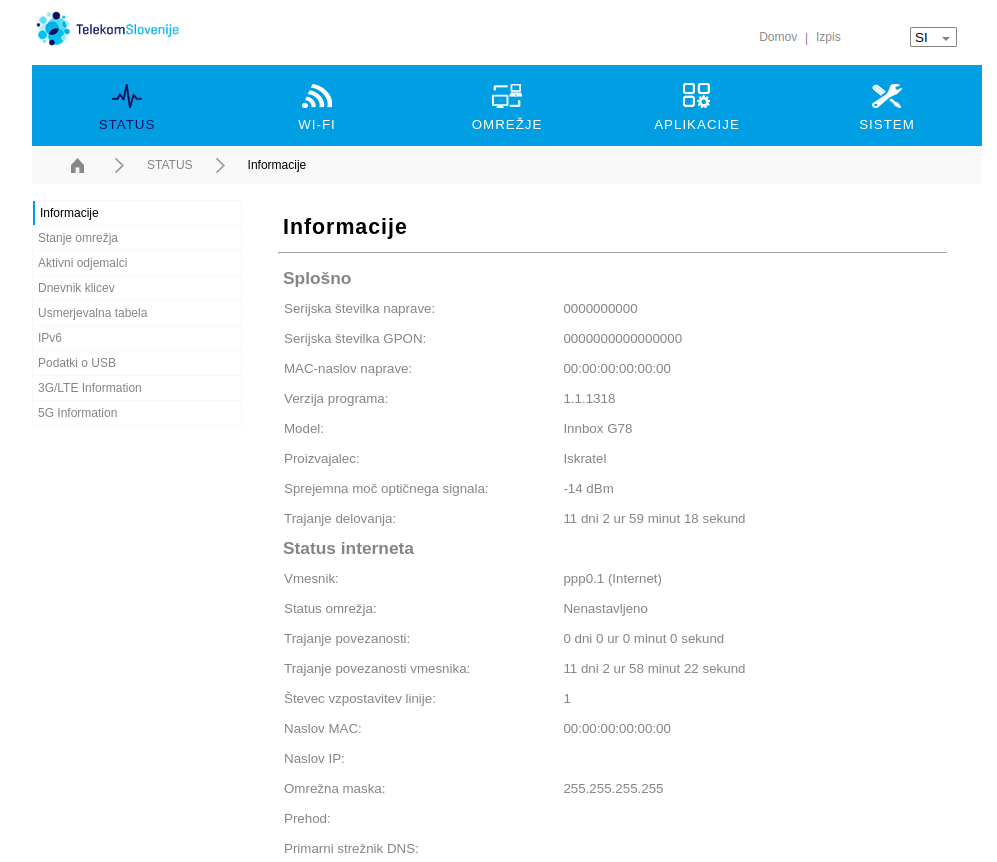
\includegraphics[scale=0.5]{slike/telekom.png}
	\captionof{figure}{Primer konfiguracijske strani za usmerjevalnike Telekoma Slovenije}
\end{center}
\newpage

% 2. Tehnologije
\section{Uporabljene tehnologije}
Tako Shedi, kot tudi RIPtide so napisani v Javi. Java omogoča dinamično
nalaganje modulov ob zagonu navideznega stroja, tudi iz zapakiranih jar
datotek. Sam RIPtide je zgrajen iz dveh glavnih delov: osprednega dela 
in aplikacijskega programskega vmesnika (v nadaljevanju API).
Poleg tega velja omeniti Shede, ki jih lahko razvije kdorkoli z uporabo
RIPtide API-ja.
\newpage

% 3. Ospredni del
\section{Ospredni del}
Ospredni del je odgovoren za konfiguracijo RIPtide-a, rokovanje z 
uporabnikovimi napravami ter pripadajočimi poverilnicami in za
nalaganje Shedov.

\subsection{Konfiguracija}
Uporabnik lahko svoje naprave shrani, in si s tem prihrani čas za morebitno
kasnejšo konfiguracijo. Poleg tega RIPtide omogoča spremembo barve vmesnika
po uporabnikovi želji.

\subsubsection{Shranjevanje podatkov}
Okoljske spremenljivke, naprave in poverilnice so zapisanje v objektu
imenovanem Workspace.

\begin{lstlisting}
@Data
public class Workspace implements Serializable {
	private Theme theme;
	private ArrayList<Credential> credentials;
	private ArrayList<Connection> connections;

	public Workspace() {
		theme = Theme.PRIMER_DARK;
		credentials = new ArrayList<>();
		connections = new ArrayList<>();
	}

	public Workspace(Theme theme, ArrayList<Credential> credentials, ArrayList<Connection> connections) {
		this.theme = theme;
		this.credentials = credentials;
		this.connections = connections;
	}
}
\end{lstlisting}
Ko uporabnik nastavitve shrani je objekt serializiran in zapisan v datoteko
na uproabnikov sistem. Datotek je lahko več, kar omogoča prilagoditev
vmesnika za različna okolja (npr. posebej za domačo in poslovno rabo).
Workspace datoteke so shranjene v JSON formatu, kar uporabnikom omogoča
enostavno izmenjavo ali prenos.

\subsubsection{Barve vmesnika}
Uporabnik lahko vmesnik prilagodi na štiri priložene teme. V prihodnosti
bo mogoče nalaganje barv iz CSS datoteke po meri.

\subsection{Upravljanje poverilnic in naprav}
Za konfiguracijo večine omrežnih naprav je potrebna avtorizacija.
RIPtide uporabnikom omogoča varno shranjevanje poverilnic na njihovem
sistemskem keyringu. Poverilnice so ob povezavi na napravo prek API-ja
podani Shedu, kar pomeni, da se razvijalci teh ne rabijo ukvarjati z
varnim hranjenjem poverilnic. Več o rokovanju z napravami v razdelku
\ref{api}. 

\subsection{Nalaganje Shedov}
\newpage

% 3. Aplikacijski programski vmesnik
\section{Aplikacijski programski vmesnik} \label{api}
\newpage

\end{document}